
\chapter{常用环境及参考文献设置}
强烈建议在使用公式、表格、定理环境时进行百度,没必要研究各种用法,只需要知道自己需要什么。因本人的论文所用表格较少,因而对表格不是很熟悉,本章对表格的介绍相应的较少。本章仅介绍本人在论文撰写过程中常用的环境以及参考文献设置。

\section{图}
图的导入需要提前准备好图片文件,最好是.png、.eps、.pdf或.jpg文件。另外,如果是从matlab导出图片文件,可使用print函数或手动导出,print函数的使用可参考“论文matlab作图程序"里的PlotToFileColorPDF.m文件。手动导出主要用于观察效果,可设置某种导出样式后导出该样式,下次使用时加载,具体可百度“matlab导出高清图片”。需要特别注意的是一定要1:1导入matlab生成的图片,并且图中文字设置好字体字号。

使用如下代码放置独立成行的图片,效果如图\ref{one_DFUAV}所示
\begin{lstlisting}
\begin{figure}[htbp]
	% 图片居中(列居中对齐)
	\centering	
	% 包含当前路径下的Fig文件夹的图片文件DFUAV_f31.png
	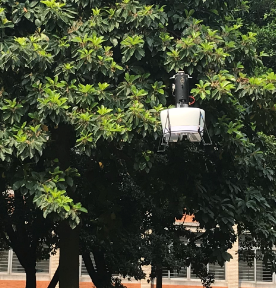
\includegraphics[scale=1]{Fig/DFUAV_f31.png} 
	% 添加标签one_DFUAV以及图标题“涵道风扇式无人机”,标题编号是自动生成的
	\caption{\label{one_DFUAV}涵道风扇式无人机} 
\end{figure}
\end{lstlisting}
其中figure为环境名,[htbp]表示将图片设置为浮动体,实际上这在.cls文件已经设置过,因而可以省略。[scale=1]表示安装1:1的比例导入图片,还可以按其他方式导入,需要时可自行百度。
\begin{figure}[htbp]
	\centering
	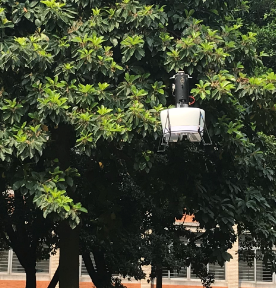
\includegraphics[scale=1]{Fig/DFUAV_f31.png}
	\caption{\label{one_DFUAV}涵道风扇式无人机}
\end{figure}

使用如下代码划分页面并排放置图\ref{Hawk}、图\ref{GTSpy}
\begin{lstlisting}
\begin{figure}[htbp]
	\centering
	\begin{minipage}[c]{0.5\textwidth} % minipage将页面划分为0.5\textwidth
		\centering
		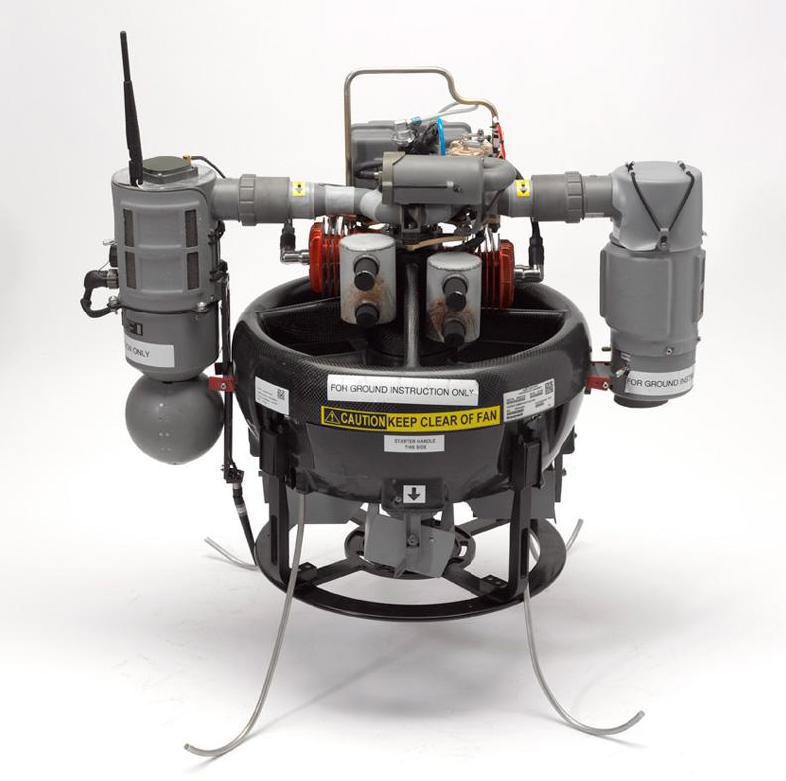
\includegraphics[width=6cm,height=6cm]{Fig/honeywell_t-hawk.jpg}
		\caption{\label{Hawk}T-Hawk}
	\end{minipage}%
	\begin{minipage}[c]{0.5\textwidth}
		\centering
		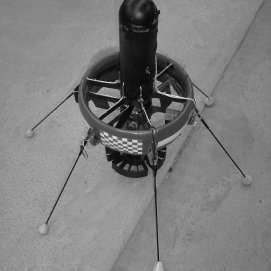
\includegraphics[width=6cm,height=6cm]{Fig/GTSpy.jpg}
		\caption{\label{GTSpy}GTSpy}
	\end{minipage}
\end{figure}
\end{lstlisting}
其中[c]表示行居中对齐。当图片大小不一但又需要1:1导入时,图标题可能行不对齐,因此可以改为如下指令:
\begin{lstlisting}
\begin{figure}[htbp]
	\centering
	\begin{minipage}[c]{0.5\textwidth}
		\centering
		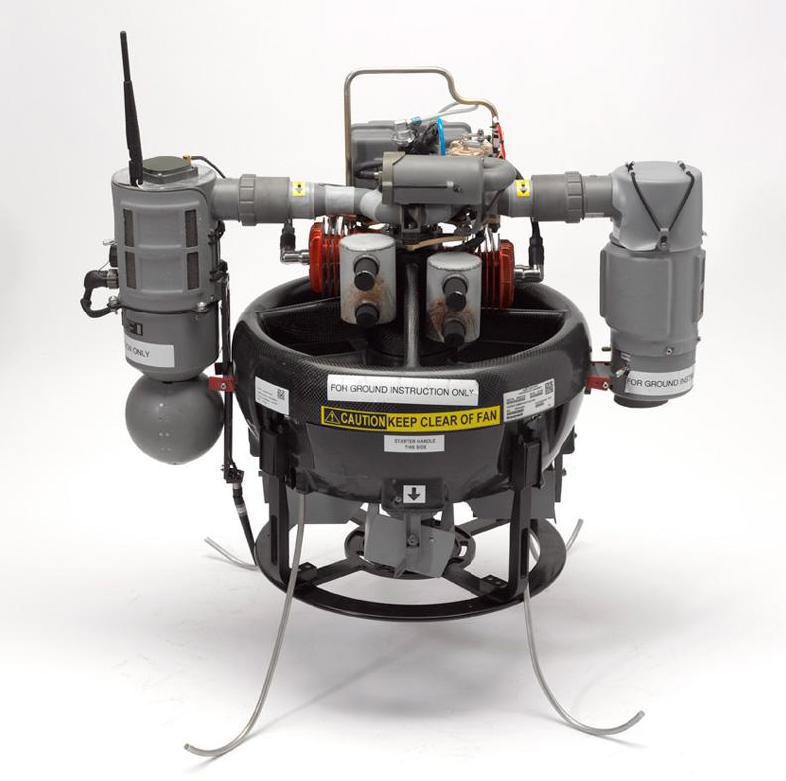
\includegraphics[scale=1]{Fig/honeywell_t-hawk.jpg} %1:1导入
	\end{minipage}%
	\begin{minipage}[c]{0.5\textwidth}
		\centering
		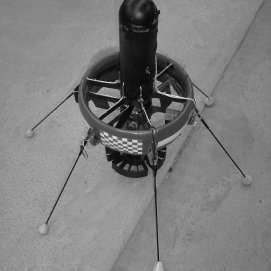
\includegraphics[scale=1]{Fig/GTSpy.jpg}
	\end{minipage}\\[1pt]
	\begin{minipage}[t]{0.5\textwidth}	% 以下为新添加页面划分,[t]表示行顶部对齐
		\caption{\label{Hawk}T-Hawk}
	\end{minipage}%
	\begin{minipage}[t]{0.5\textwidth}
		\caption{\label{GTSpy}GTSpy}
	\end{minipage}%
\end{figure}
\end{lstlisting}
\begin{figure}[htbp]
	\centering
	\begin{minipage}[c]{0.5\textwidth}
		\centering
		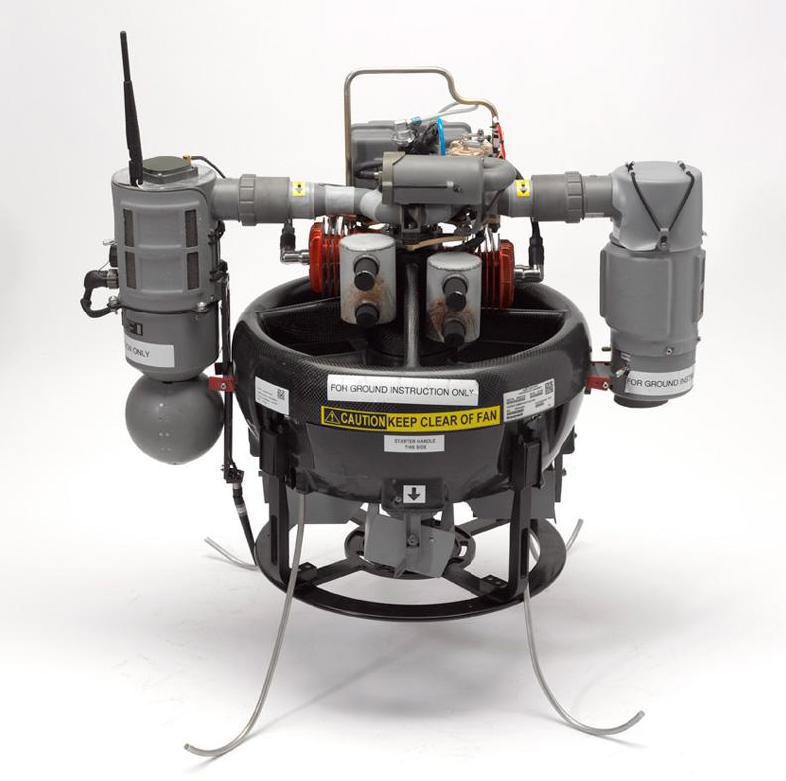
\includegraphics[width=6cm,height=6cm]{Fig/honeywell_t-hawk.jpg}
		\caption{\label{Hawk}T-Hawk}
	\end{minipage}%
	\begin{minipage}[c]{0.5\textwidth}
		\centering
		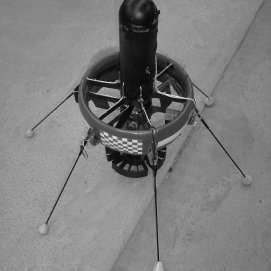
\includegraphics[width=6cm,height=6cm]{Fig/GTSpy.jpg}
		\caption{\label{GTSpy}GTSpy}
	\end{minipage}
\end{figure}
\section{表}
本节仅展示使用常见的三线表
\begin{lstlisting}
\begin{table}
	\caption{\label{TDF_para}涵道模型参数}	%表题在上
	\centering	% 表居中
	\small	% 表内字体小一号(即设置成和表题字号一致)
	\begin{tabular}{cccc}	% cccc表示4列并居中,若列之间需要分隔符则设置为|c|c|c|c|
		\hline	% \hline表示横线。列之间的元素用&分隔,\tabularnewline表示换行
		参数符号 & 数值 & 参数符号 & 数值 \tabularnewline 
		\hline 
		$I_x$ & $054593$ 		   & $I_y$ & $0.017045         $ \tabularnewline
		$l_1$ & $0.0808\,\text{m}$ & $l_2$ & $0.175\,\text{m}  $ \tabularnewline 
		$l_4$ & $0.2415\,\text{m}$ & $l_5$ & $0.1085\,\text{m} $ \tabularnewline
		\hline 
	\end{tabular}
\end{table}
\end{lstlisting}
\begin{table}
	\caption{\label{TDF_para}涵道模型参数}
	\centering
	\small 
	\begin{tabular}{cccc}
		\hline 
		参数符号 & 数值                & 参数符号 & 数值                 \tabularnewline
		\hline 
		$I_x$   & $054593$ 		     & $I_y$   & $0.017045         $ \tabularnewline
		$l_1$   & $0.0808\,\text{m}$ & $l_2$   & $0.175\,\text{m}  $ \tabularnewline 
		$l_4$   & $0.2415\,\text{m}$ & $l_5$   & $0.1085\,\text{m} $ \tabularnewline
		\hline 
	\end{tabular}
\end{table}

\section{公式}
除了前面讲行内公式,常用的还有行间公式。公式中的数学符号可自行百度,本章仅介绍常用的几种公式环境。

单独成行的行间公式在 \LaTeX{} 里由equation 环境包裹。equation 环境为公式自动生成一个编号,这个编号可以用\textbackslash{}label 和\textbackslash{}ref 生成交叉引用,amsmath 宏包的\textbackslash{}eqref 可为引用自动加上圆括号;如式\eqref{eq_1}所示。
\begin{lstlisting}
\begin{equation}
	a+b=c	\label{eq_1}
\end{equation}
\end{lstlisting}
\begin{equation}
	a+b=c	\label{eq_1}
\end{equation}
若不需要编号则加星号,改为
\begin{lstlisting}
\begin{equation*}
	a+b=c
\end{equation*}
\end{lstlisting}
其他环境类似。当使用 \texttt\$ 开启行内公式输入,或是使用{equation} 环境时,\LaTeX\ 就进入了数学模式。
数学模式相比于文本模式有以下特点:
\begin{enumerate}
	\item 数学模式中输入的空格被忽略。数学符号的间距默认由符号的性质(关系符号、运算符等)决定。
	需要人为引入间距时,使用 \textbackslash{}{quad} 和 \textbackslash{}{qquad} 等命令。
	\item {不允许有空行(分段)}。行间公式中也无法用 $ \verb|\\|$命令手动换行。排版多行公式需要用到 其他各种环境。
	\item 所有的字母被当作数学公式中的变量处理,字母间距与文本模式不一致,也无法生成单词之间的空格。
	如果想在数学公式中输入正体的文本,简单情况下可用 \textbackslash{}{mathrm} 命令。
	或者用 {amsmath} 提供的 \textbackslash{}{text} 命令(仅适合在公式中穿插少量文字。如果你的情况正好相反,需要在许多文字中穿插使用公式,则应该像正常的行内公式那样用,而不是滥用 \textbackslash{}{text} 命令)。
\end{enumerate}	

实际上更常用的的是多行公式,不需要对齐的公式组可以使用gather环境,需要对齐的公式组用align 环境。
长公式内可用$ \verb|\\|$ 换行。

如果需要罗列一系列公式,并令其按照等号对齐,可用align 环境,它将公式用\& 隔为两部分并对齐。分隔符通常放在等号左边:
\begin{lstlisting}
\begin{align}
	a & = b + c \\
	& = d + e
\end{align}
\end{lstlisting}
\begin{align}
a & = b + c \\
& = d + e
\end{align}
align 环境会给每行公式都编号。

如果不需要按等号对齐,只需罗列数个公式,可用gather环境:
\begin{lstlisting}
\begin{gather}
	a  = b + c \notag \\
	f = d + e 
\end{gather}
\end{lstlisting}
\begin{gather}
	a  = b + c \notag  \\
	f = d + e 
\end{gather}
gather 环境同样会给每行公式都编号,如果某行不需要编号可在行末用\textbackslash{}notag 仅去掉某行的编号。

align 和gather 有对应的不带编号的版本align* 和gather*。

另一个常见的需求是将多个公式组在一起公用一个编号,编号位于公式的居中位置。为此,
amsmath 宏包提供了诸如aligned、gathered 等环境,与equation 环境套用。以-ed 结尾的
环境用法与前一节不以-ed 结尾的环境用法一一对应。我们仅以aligned 举例:
\begin{lstlisting}
\begin{equation}
	\begin{aligned}
		a &= b + c \\
		d &= e + f + g \\
		h + i &= j + k \\
		l + m &= n
	\end{aligned}
\end{equation}
\end{lstlisting}
\begin{equation}
	\begin{aligned}
		a &= b + c \\
		d &= e + f + g \\
		h + i &= j + k \\
		l + m &= n
	\end{aligned}
\end{equation}
split 环境和aligned 环境用法类似,也用于和equation 环境套用,区别是split 只能
将每行的一个公式分两栏,aligned 允许每行多个公式多栏。

分段函数通常用amsmath 宏包提供的cases 环境,可参考文献\parencite{_c}

amsmath 宏包还直接提供了多种排版矩阵的环境,包括不带定界符的matrix,以及带各种定界符的矩阵pmatrix、bmatrix、Bmatrix、vmatrix、Vmatrix。
其中中括号版的bmatrix最常用。这些矩阵环境需要在公式中使用,比如 align 环境。
\begin{lstlisting}
A= \begin{bmatrix}
		x_{11} & x_{12} & \ldots & x_{1n} \\
		x_{21} & x_{22} & \ldots & x_{2n} \\
		\vdots & \vdots & \ddots & \vdots \\
		x_{n1} & x_{n2} & \ldots & x_{nn}
	\end{bmatrix}
\end{gather}
\end{lstlisting}
\begin{gather}
\bm{A}= \begin{bmatrix}
	x_{11} & x_{12} & \ldots & x_{1n} \\
	x_{21} & x_{22} & \ldots & x_{2n} \\
	\vdots & \vdots & \ddots & \vdots \\
	x_{n1} & x_{n2} & \ldots & x_{nn}
   \end{bmatrix}
\end{gather}	
其中矩阵/向量加粗使用\textbackslash{}bm\{\}命令。另外还可以使用array环境排版矩阵,类似tabular环境,用$ \verb|\\|$ 和\& 用来分隔行和列,这里不再赘述。	
\begin{lstlisting}
\begin{array }[外部对齐tcb]{列对齐lcr}
	行列内容
\end{array}
\end{lstlisting}

另外注意排版分式时,有两种方法:\textbackslash{}frac或者\textbackslash{}dfrac,效果分别为$ \frac{1}{2} $和$ \dfrac{1}{2} $。以上介绍的数学环境中,空格可参考文献\parencite{_c},例如常用\textbackslash{}quad。
\section{定理}
在scutthesis.cls文件536行开始,已经用\textbackslash{}newtheorem命令定义了几种定理环境,包括:定义、假设、定理、结论、引理、公理、推论、性质等等,统称定理环境,关于\textbackslash{}newtheorem的用法,可参考\cite{_c}或自行百度。要下面提供几个例子,在横线之间的深色区域是代码,效果在相应下方表示:
\begin{lstlisting}
\begin{assumption}
	加权矩阵${{\bm{W}}_{1}}$和 ${{\bm{W}}_{2}}$ 是对称矩阵,且$ {{\bm{W}}_{2}}$非奇异。	\label{assum_dca1}
\end{assumption}
\end{lstlisting}
\begin{assumption}
	加权矩阵${{\bm{W}}_{1}}$和 ${{\bm{W}}_{2}}$ 是对称矩阵,且$ {{\bm{W}}_{2}}$非奇异。	\label{assum_dca1}
\end{assumption}

定理用法和假设类似:
\begin{lstlisting}
\begin{theorem}
	如果假设\ref{assum_dca1}成立,$\bm{F}$满足式\eqref{eq_F}的定义,且${{\bm{W}}_{1}}$非奇异,则有$0\le e \left( \bm{F} \right) < 1$,其中$e \left( \bm{F} \right)$是 $\bm{F}$的特征值。	\label{the_dca2}
\end{theorem}
\end{lstlisting}
\begin{theorem}
	如果假设\ref{assum_dca1}成立,$\bm{F}$满足上式的定义,且${{\bm{W}}_{1}}$非奇异,则有$0\le e \left( \bm{F} \right) < 1$,其中$e \left( \bm{F} \right)$是 $\bm{F}$的特征值。	\label{the_dca2}
\end{theorem}

定理环境的编号可自定义,但通常不需要再进行设置,因为模板文件scutthesis.cls文件已经定义好。
\section{参考文献}
通常学位论文参考文献是基于BibTeX进行的,本模板最大的改进就是引入BibLaTeX。关于这部分知识可参考文献\cite{_c}的第六章,6.1节参考文献和BIBTEX工具。

参考文献引用和著录是基于ZOTERO这个软件进行的。视频教程见\parencite{_e}。此外,为了符合毕业论文撰写规范,需设置参数。按照视频教程安装完必要的插件(如Better BibTeX)后,在编辑->首选项进行设置。图\ref{op1}到图\ref{op11}所示的是我的zotero软件设置。

在zotero软件点击文件->导出文献库,如图\ref{output}所示,再在导出对话框图\ref{output_format}选择导出格式为Better BibLaTeX,同时勾选Keep updated选项保持自动更新,再点击ok,在弹出的对话框图\ref{output_name}确定保存路径和文件名,例如我的是MyLibrary.bib,这也是我整个读书生涯的文献库bib文件。如果写小论文的话通常导出格式是BibTeX或者Better BibTeX(这里按照期刊的要求来即可,文献管理软件的好处就是快速自动生成一个文件库)。关于BibTeX和BibLaTeX的区别这里不做展开。

得到文献库后,在scutthesis.tex文件第九行使用\textbackslash{}addbibresource命令,添加文献库。引用某文献时秩序在zotero选中某文献条目,然后按Ctrl+Shift+C,复制引用关键字(Citation Key)到剪切板。然后在tex文件编辑界面直接粘贴,默认的时上标形式,若需要非上标形式,可以改为\textbackslash{}parencite{XXXX},其中XXXX是Citation Key。这里的操作和认为设置的首选项参数有关,需要在编辑->首选项->导出界面的默认格式一栏选中相应的项,同时在编辑->首选项->高级->快捷键设置为默认值。

值得注意的是,在毕业论文撰写时,在编辑->首选项->Better BibLTeX->Fields中,Fields to omit from export填month,abstract,note,extra,file,keywords,type,url,doi,就是在参考文献著录中排除这些多余的项,避免过于复杂。而在写本模板使用说明时,没有排除url,因为很多参考资料是网页。

\begin{figure}
	\centering
	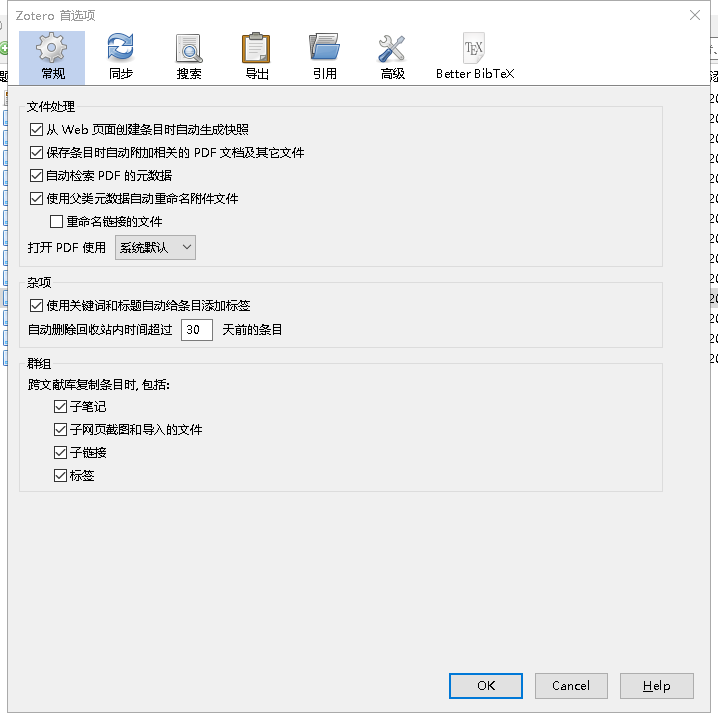
\includegraphics[scale=0.8]{Fig/zotero1.png}
	\caption{\label{op1}常规}
\end{figure}
\begin{figure}
	\centering
	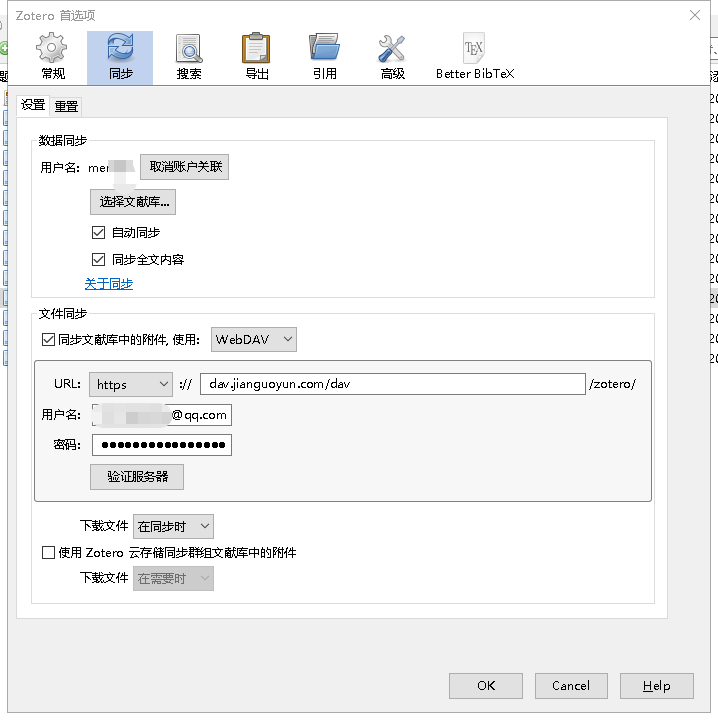
\includegraphics[scale=0.8]{Fig/zotero2.png}
	\caption{\label{op2}同步1}
\end{figure}
\begin{figure}
	\centering
	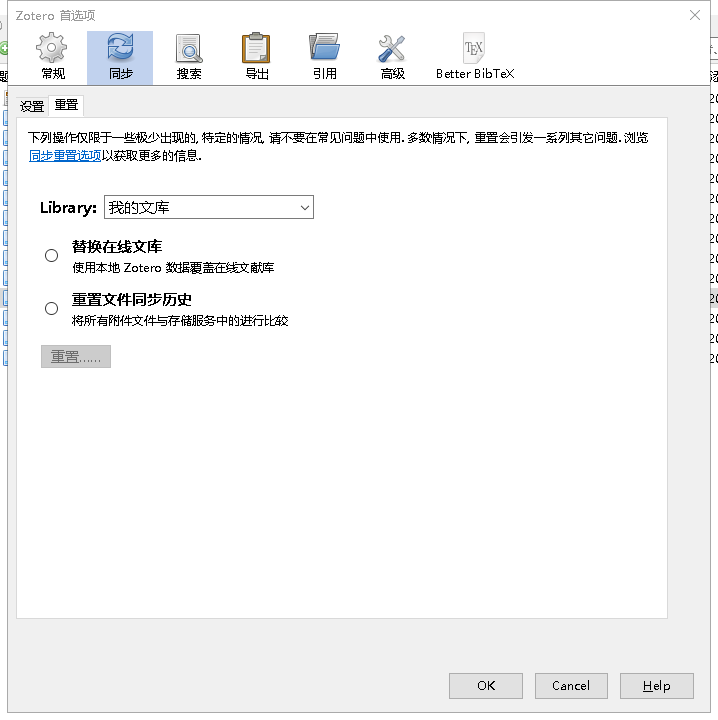
\includegraphics[scale=0.8]{Fig/zotero3.png}
	\caption{\label{op3}同步2}
\end{figure}
\begin{figure}
	\centering
	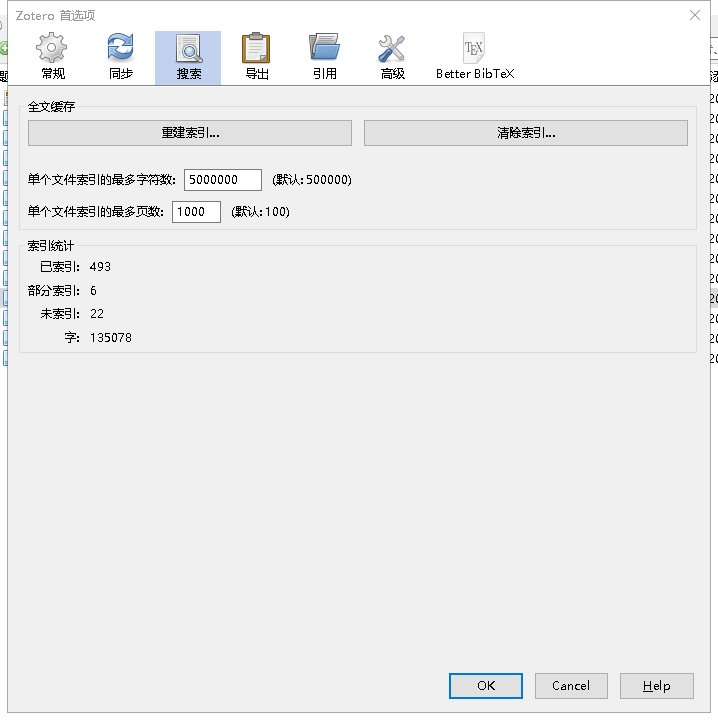
\includegraphics[scale=0.8]{Fig/zotero4.png}
	\caption{\label{op4}搜索}
\end{figure}
\begin{figure}
	\centering
	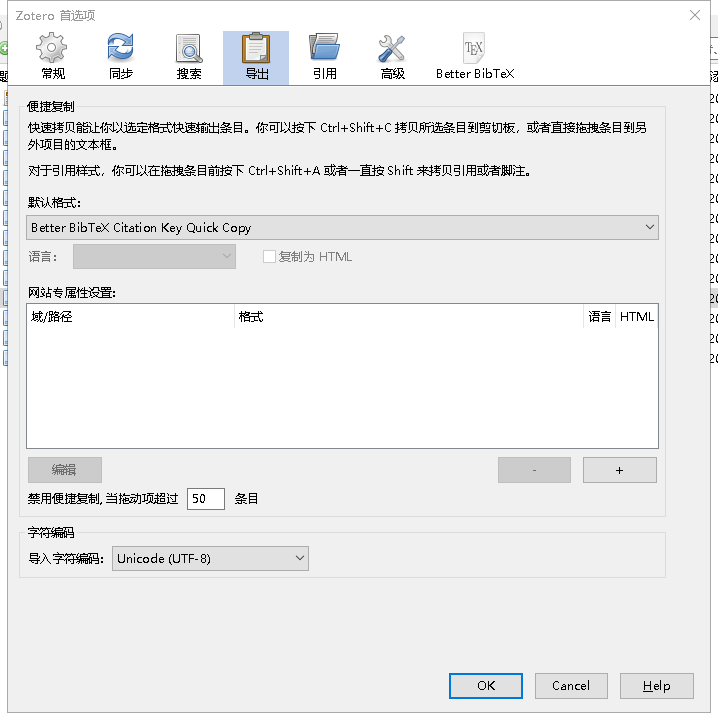
\includegraphics[scale=0.8]{Fig/zotero5.png}
	\caption{\label{op5}导出}
\end{figure}
\begin{figure}
	\centering
	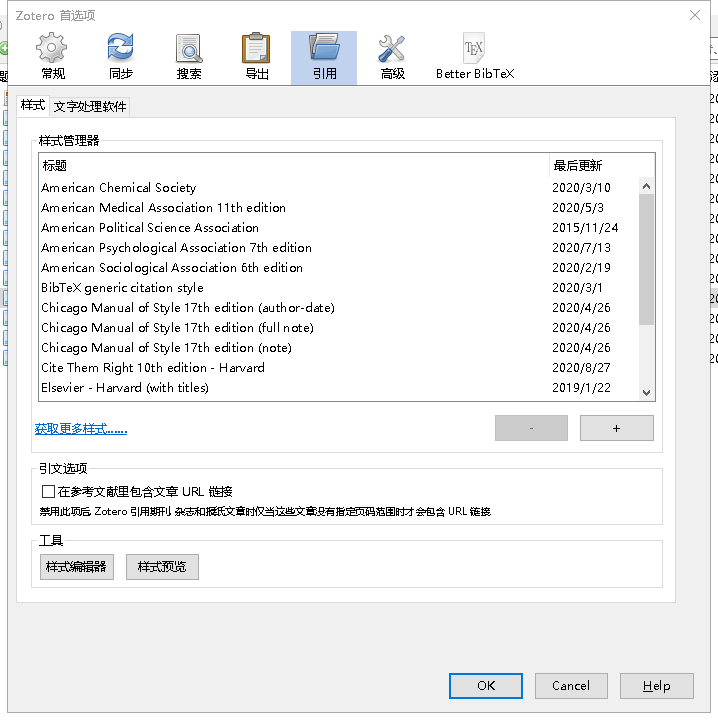
\includegraphics[scale=0.8]{Fig/zotero6.png}
	\caption{\label{op6}引用}
\end{figure}
\begin{figure}
	\centering
	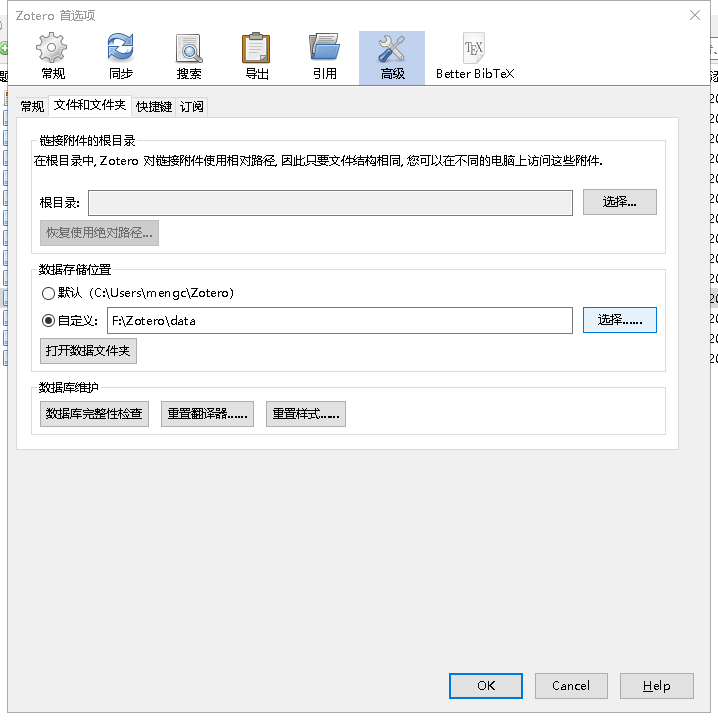
\includegraphics[scale=0.8]{Fig/zotero7.png}
	\caption{\label{op7}高级1}
\end{figure}
\begin{figure}
	\centering
	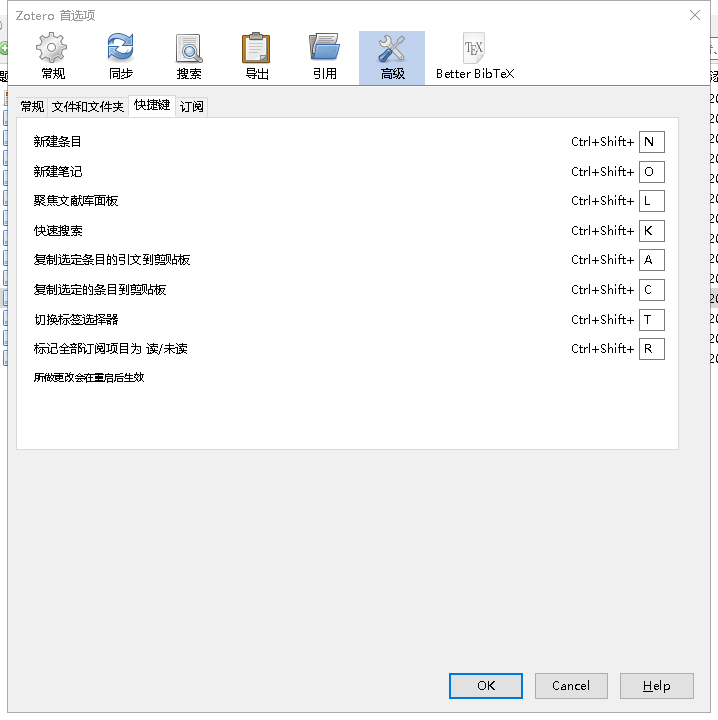
\includegraphics[scale=0.8]{Fig/zotero8.png}
	\caption{\label{op8}高级2}
\end{figure}
\begin{figure}
	\centering
	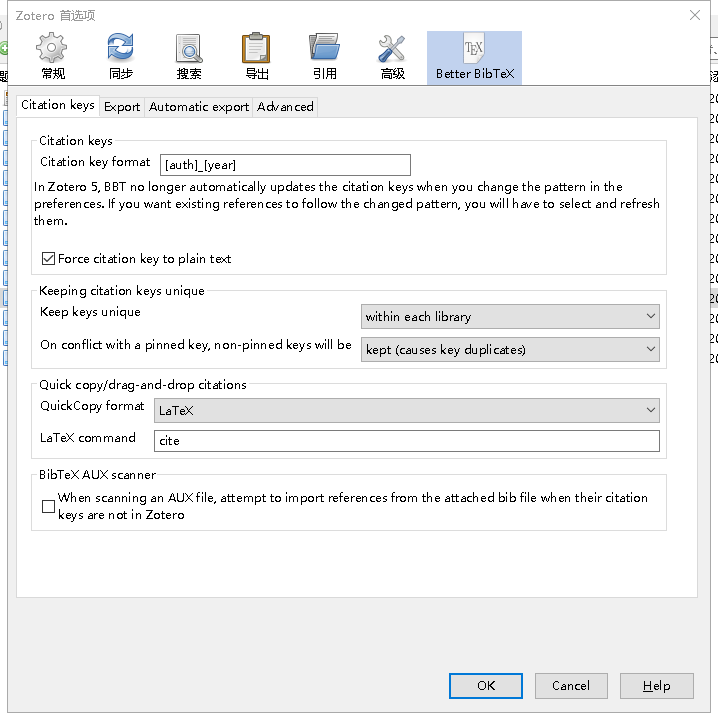
\includegraphics[scale=0.8]{Fig/zotero9.png}
	\caption{\label{op9}Better BibTeX1}
\end{figure}
\begin{figure}
	\centering
	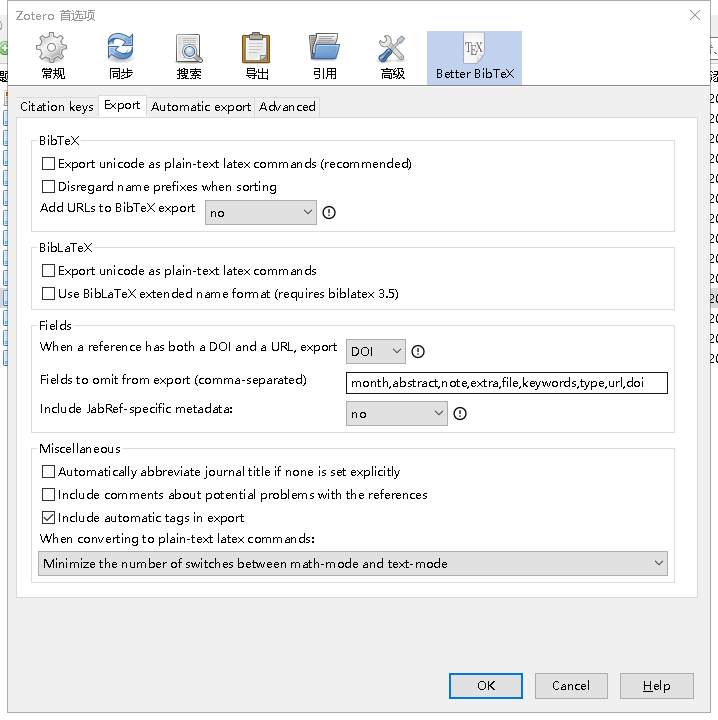
\includegraphics[scale=0.8]{Fig/zotero10.png}
	\caption{\label{op10}Better BibTeX2}
\end{figure}
\begin{figure}
	\centering
	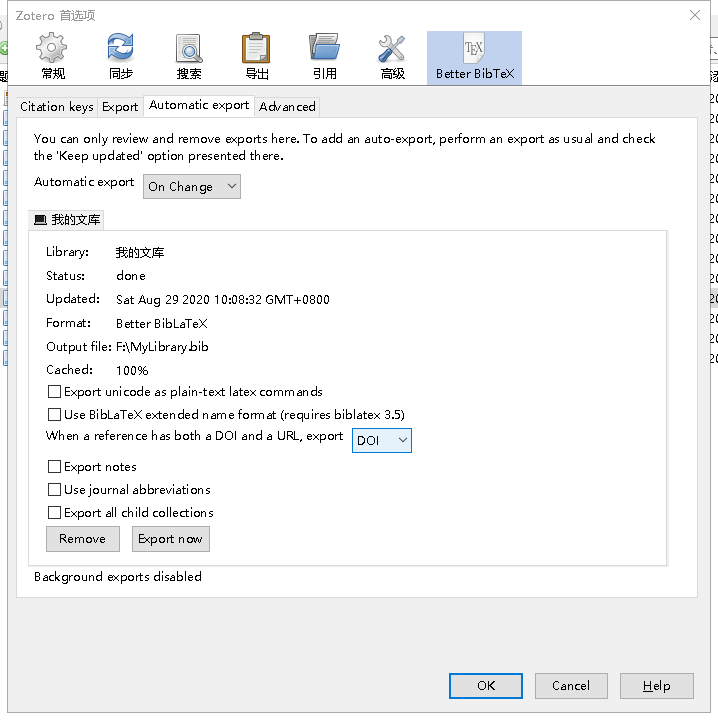
\includegraphics[scale=0.8]{Fig/zotero11.png}
	\caption{\label{op11}Better BibTeX3}
\end{figure}

\begin{figure}[htbp]
	\centering
	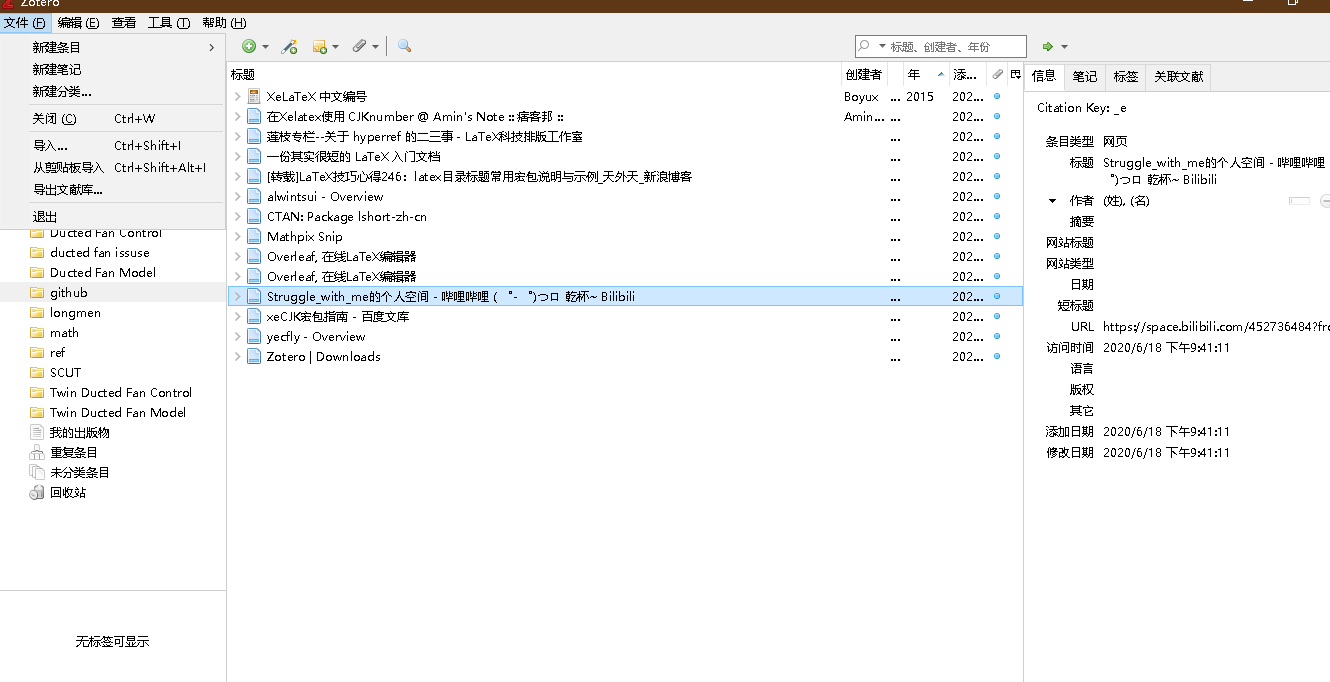
\includegraphics[scale=0.42]{Fig/zotero12.png}
	\caption{\label{output}导出文献库}
\end{figure}

\begin{figure}[htbp]
	\centering
	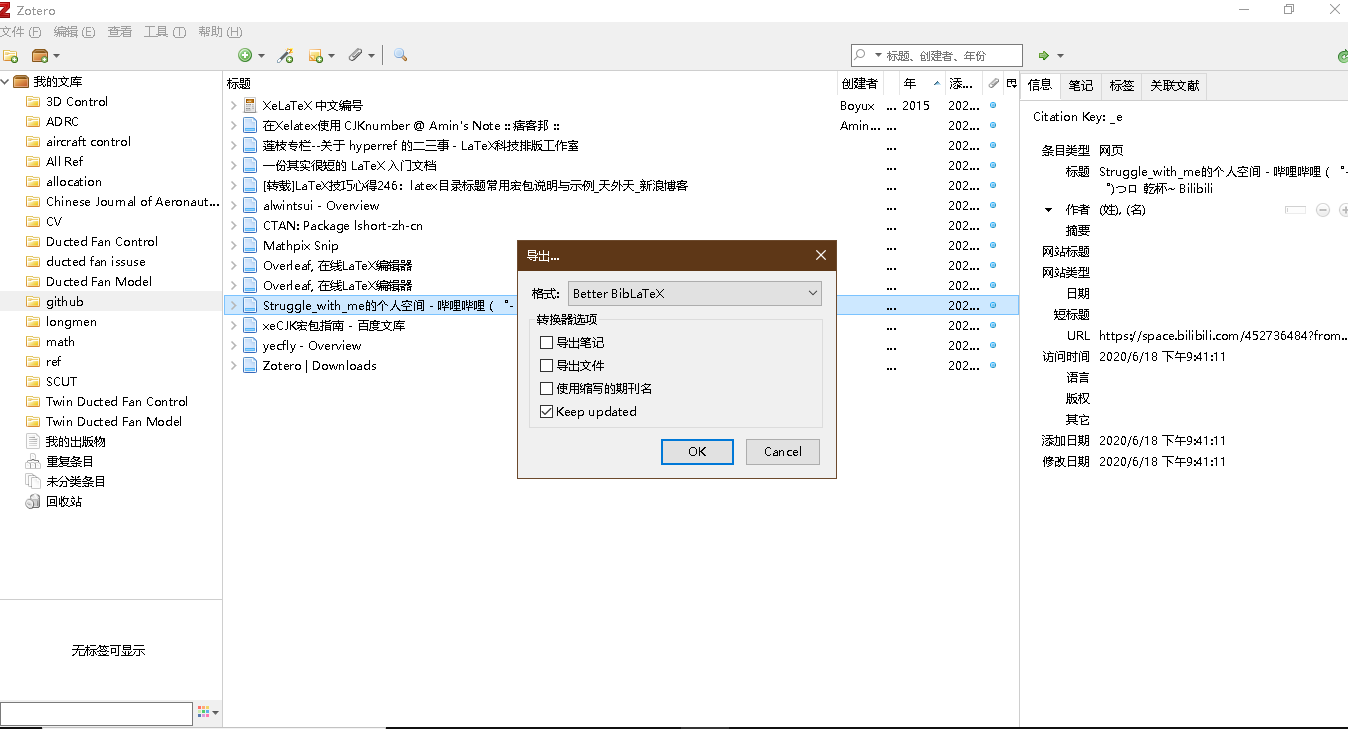
\includegraphics[scale=0.42]{Fig/zotero13.png}
	\caption{\label{output_format}导出格式}
\end{figure}

\begin{figure}[htbp]
	\centering
	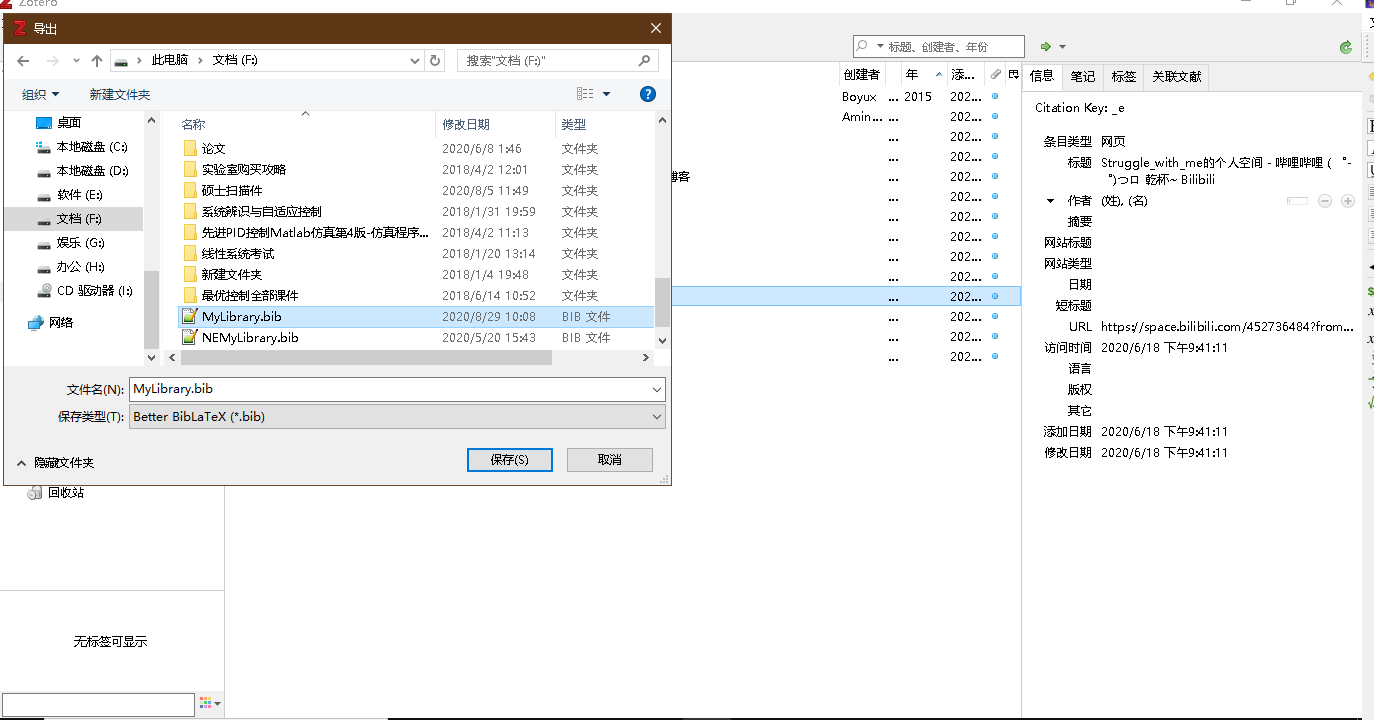
\includegraphics[scale=0.42]{Fig/zotero14.png}
	\caption{\label{output_name}导出文件名}
\end{figure}







